\documentclass[11pt,a4paper]{article}
\usepackage{a4wide,url,graphicx,wrapfig}
\usepackage[utf8]{inputenc}
\usepackage[main=ngerman,russian]{babel}

\parindent0pt
\parskip3pt

\title{Der Mensch und das technische System} 

\author{Nikolay Shpakovsky, Minsk}

\date{20. Januar 2003}

\begin{document}
\maketitle

\begin{quote}
  Der russische Originaltext besteht aus zwei Teilen, die hier zusammengefasst
  sind
  
  Teil 1: \url{http://www.gnrtr.ru/Generator.html?pi=201&cp=3}\\
  Teil 2: \url{http://www.gnrtr.ru/Generator.html?pi=200&cp=3}
\end{quote}

\section*{Ist der Mensch Teil des technischen Systems oder nicht?}

\begin{flushright}
 \ldots\ die letzten Worte des Buches des Propheten Lustrog lauten:\\ „Alle
 wahren Gläubigen öffnen ihre Eier\\ an dem Ende, an dem es bequemer
 ist“. \\ Jonathan Swift, Gulliver's Reisen.
\end{flushright}

\section*{Einleitung}
Die Theorie des Lösens von Erfindungsaufgaben (TRIZ), vom talentierten
Ingenieur, Erfinder und genialen Ausdenker G.S. Altshuller entwickelt, ist
weit bekannt und zur heutigen Zeit zweifellos das wirksamste Werkzeug zur
Lösung von Ingenieuraufgaben. Eine große Zahl von Materialien ist dazu in
Russisch und Englisch veröffentlicht worden, in denen das Wesen der Theorie
für eine erste Einführung ausreichend umfassend dargestellt wird.  Die beste
russischsprachige Ressource ist die Website des Minsker
OTSM-TRIZ-Zentrums\footnote{\url{http://www.trizminsk.org}}, die bestes
Englischsprachige der Amerikanische
TRIZ-Journal\footnote{\url{http://www.triz-journal.com}}. Wenn man TRIZ aus
Büchern und Artikel studiert hat, kann man leicht andere unterrichten -- das
Material ist so reichhaltig und faszinierend, dass das Interesse an einer
Beschäftigung mit dem Stoff gewährleistet ist.

Für ein tieferes Verständnis der TRIZ ist jedoch eine sorgfältige Abwägung des
vorgestellten Materials erforderlich, vor allem der Konzepte und Begriffe der
TRIZ.  Vieles in TRIZ ist als Material zur Anregung zum weiteren Nachdenken
beschrieben und nicht als Menge von Informationen zum einfachen
Auswendiglernen.

Als ich für SAMSUNG als TRIZ-Berater arbeitete, musste ich alles, was ich
bisher über die TRIZ wusste, von neuem und ernsthaft überdenken. Bei der
Lösung technischer Aufgaben, der Umgehung von Patenten konkurrierender
Unternehmen und der Erarbeitung von Prognosen der Entwicklung technischer
Systeme war es sehr wichtig, den tieferliegenden Inhalt jedes Begriffs der
TRIZ genauer zu verstehen, um die TRIZ-Instrumente mit maximaler Effektivität
anzuwenden.

Eines der grundlegenden Konzepte in der TRIZ und eines der wichtigsten
Bindeglieder aller seiner Instrumente ohne Ausnahme ist der Begriff
„Technisches System“. Dieser Begriff wird in der klassischen TRIZ ohne
Definition eingeführt, als Ableitung des Begriffs „System“. Aber bei näherer
Betrachtung wird klar, dass dieser Begriff -- „Technisches System“ -- eine
weitere Konkretisierung erfordert. Zu Gunsten einer solchen Behauptung spricht
zum Beispiel der semantische Aspekt. Der Begriff „technisches System“ wird auf
zwei Arten vom Russischen ins Englische übersetzt: „Tecnical System“ und
„Engineering System“.  Mit einer beliebigen Suchmaschine im Internet kann man
sich leicht überzeugen, dass diese beiden Konzepte von Fachleuten, die in der
TRIZ aktiv sind, fast gleichwertig verstanden werden. Oder nehmen Sie zum
Beispiel das Glossar von Victor
Fey\footnote{\url{http://www.triz-journal.com/archives/2001/03/a/index.htm}},
in dem einfach keines der beiden Konzepte erläutert wird.

In diesem Artikel habe ich versucht, mein Verständnis des Begriffs
„technisches System“ zu beschreiben, das sich schrittweise entwickelt hat,
wenn ich zur Lösung einer konkreten Aufgabe die vollständige Zusammensetzung
eines minimalen technisch arbeitsfähigen Systems herausfinden musste.

\section*{Ein Versuch, den Begriff „technisches System“ zu analysieren}

Lasst uns zunächst einmal überlegen, was ein System überhaupt ist. Es gibt
viele verschiedene Systemdefinitionen. Die einprägsamste, abstrakteste, und
damit absolut erschöpfende Definition, die aber von geringem praktischen
Nutzen ist, hat B. Gaines [1] gegeben: \textbf{„Ein System ist das, was wir
  als ein System definieren“}.  In der Praxis wird die Systemdefinition von
A. Bogdanov am häufigsten verwendet [2]: \textbf{“Ein System ist eine Menge
  miteinander verbundener Elemente mit einer gemeinsamen (System-)Eigenschaft,
  die nicht auf Eigenschaften dieser Elemente reduzierbar ist“}.

Was aber ist ein “Technisches System“? 

Leider ist das Konzept des „Technischen Systems“ bei G. Altschuller nicht
direkt definiert. Aus dem Kontext wird klar, dass es sich um eine Art System
handelt, das mit Technik technischen Objekten zu tun hat. Als indirekte
Definition eines technischen Systems (TS) können drei von Altschuller
formulierte Gesetze oder vielmehr drei Bedingungen dienen, die für deren
Existenz erfüllt sein müssen [3]:
\begin{itemize}\itemsep0pt
\item[1.] Das Gesetz der Vollständigkeit der Teile des Systems. 
\item[2.] Das Gesetz der „Energieleitfähigkeit“ des Systems. 
\item[3.] Das Gesetz der Abstimmung der Rhythmik der Teile des Systems.
\end{itemize}
Nach dem Gesetz der Vollständigkeit der Teile des Systems umfasst jedes TS
mindestens vier Teile: Antrieb, Transmission, Arbeitskörper und
Steuerungssystem.
\begin{center}
 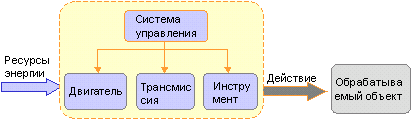
\includegraphics[width=.6\textwidth]{mts-1.png}\\ Minimale Struktur eines
 funktionsfähigen technischen Systems nach G. Altschuller.
\end{center}
Das heißt, es gibt ein System, eine Maschine, die aus technischen Objekten,
Untersystemen besteht, das die geforderte Funktion erfüllen kann. Es umfasst
wenigstens das Arbeitsorgan, die Transmission und den Antrieb. Alles, was den
Betrieb dieser Maschine steuert, wird im „Steuerungssystem“ oder dem
unverständlichen „kybernetischen Teil“ [4] zusammengefasst.

Wichtig ist hier das Verständnis, dass das TS geschaffen wurde, um eine
bestimmte Funktion auszuführen. Wahrscheinlich sollte das so verstanden
werden, dass ein minimal funktionsfähiges TS diese Funktion zu jeder Zeit
ausführen kann, ohne zusätzliche Ergänzungen. Ansätze zur Definition eines
technischen Systems werden in dem Buch „Suche nach neuen Ideen“ [5]
vorgestellt, wo eine Definition eines „sich entwickelnden technischen Systems“
gegeben wird. Diese Frage wird von V. Korolev in seinen interessanten Studien
[6,7] aufgegriffen. Einige kritische Anmerkungen dazu sind in den Materialien
von N. Matvienko [8] zu finden. Die Definition des Begriffs „technisches
System“ selbst bezogen auf die TRIZ wird in dem Buch [9] von Yu. Salamatov
beschrieben: 
\begin{quote}\bf
  Ein technisches System ist eine Menge geordnet interagierender Elemente mit
  Eigenschaften, die nicht auf die Eigenschaften einzelner Elemente
  zurückzuführen sind, und die dazu bestimmt ist, bestimmte nützliche
  Funktionen zu erfüllen. 
\end{quote}
In der Tat hat der Mensch irgendwelche Bedürfnisse, zu deren Befriedigung
irgendeine Funktion ausgeführt werden muss. Das heißt, man muss irgendwie ein
System organisieren, das diese Funktion ausführt -- das „Technische System“ --
und das Bedürfnis zu befriedigen.

Was verwundert an der obigen Definition des technischen Systems? Die nicht
ganz klare Wendung „ist bestimmt für“. Wahrscheinlich sind hier nicht die
Wünsche von irgendjemandem wichtiger, sondern die objektive Fähigkeit, die
geforderte Funktion zu erfüllen.  
\begin{quote}\it
  Wozu dient zum Beispiel ein Metallzylinder mit einer axialen Bohrung mit
  variablem Durchmesser und Gewinde an einem Ende?

  Es ist praktisch unmöglich, diese Frage zu beantworten. Die Diskussion
  verschiebt sich sofort auf die Ebene der Frage „wo könnte man das
  anwenden?“.
\end{quote}
Aber kann man, wenn man diese Definition benutzt, sagen: das ist noch kein
Technisches System, aber von diesem Moment an -- nun ist es ein Technisches
System? Es heißt dazu wie folgt: “... ein TS erscheint, sobald ein technisches
Objekt die Fähigkeit erlangt, die Nützliche Hauptfunktion ohne den Menschen
auszuführen“. Und weiter heißt es, dass einer der Tendezen der Entwicklung TS
die Entfernung des Menschen aus dem TS ist. Das heißt, auf irgendeiner Etappe
der Entwicklung des TS ist der Mensch Teil davon. Oder nicht?
Nicht verständlich ...  
\begin{quote}\it
  Wahrscheinlich werden wir nichts verstehen, wenn wir auf die folgende Frage
  keine Antwort finden: Ist der Mensch Teil des technischen Systems oder
  nicht?
\end{quote}
Wenn ich bekannte TRIZniks befrage, erhalte ich eine ziemlich breite Palette
von Antworten: von einem entschiedenen „Nein“, unterstützt durch Hinweise auf
Koryphäen, bis zu einem zögerlichen „Ja, wahrscheinlich“.

Die originellste der Antworten: Wenn sich ein Auto gleichmäßig und geradlinig
bewegt, dann ist der Mensch nicht Teil dieses technischen Systems, aber sobald
das Auto beginnt, um eine Kurve zu fahren, so wird der Mensch sofort sein
notwendiger und nützlicher Teil.

Was haben wir dazu in der Literatur? Salamatov [9, Abschnitt 4.3] gibt ein
Beispiel, in welchem ein Mann mit der Hacke kein TS ist. Zumal die Hacke
selbst auch kein Technisches System ist. Aber Pfeil und Bogen sind ein TS.

Aber was ist der Unterschied zwischen einer Hacke und einem Bogen? Der Bogen
haben einen Energiespeicher - die Bogensehne und eine flexible Stange, bei
einer guten Hacke biegt sich der Stiel ebenfalls beim Schwingen, was beim
Abwärtsbewegen die Stoßkraft erhöht. Sie biegt sich nur ein wenig, aber uns
geht es ums Prinzip. Mit dem Bogen wird in zwei Phasen gearbeitet: Zuerst
spannen, dann loslassen -- mit einer Hacke auch. Warum dann so eine
Ungerechtigkeit?

Versuchen wir es herauszufinden. 

Ist ein angespitzter Holzstab ein technisches System? Es sieht nicht danach
aus.  Ein Kugelschreiber? Wahrscheinlich ein TS, und ein ziemlich
kompliziertes. Und ein Drucker?  Zweifelsohne ein TS.

Und einen Bleistift? Wer weiß ...? Wohl so: sowohl als auch. Vielleicht
sollten wir ihn “Einfaches Technisches System“ nennen? Ein Schreibgriffel aus
Blei oder Silber? Eine Frage ...  Kein einfaches Holzstück mehr, es ist
immerhin aus einem edlen Metall, aber bis zum Kugelschreiber ist es noch weit.

Ein moderner Kapillarschreiber, ein Bleistift, ein angespitzter Stab und der
Schreibkopf eines Druckers, was haben sie gemeinsam? Eine gewisse nützliche
Funktion, die sie im Prinzip ausführen können: „eine Spur auf einer Oberfläche
hinterlassen“.

„Der langlebige Timoschka läuft auf einem schmalen Pfad. Seine Fußabdrücke
sind Ihre Werke“. Erinnern Sie sich an dieses Rätsel? Gemeint ist ein
Bleistift.  Aber auch ein Stock, ein Schreibgriffel aus Blei oder Silber, ein
Stift, Marker, Drucker, eine Druckerpresse. Was für eine Auswahl! Und die
Reihung ist logisch ...

Wirklich, es stellt sich wieder eine Frage. 

Wenn alle diese Objekte die gleiche Funktion erfüllen können, dann sind das
alles -- Technische Systeme. Und mann muss Sie nicht in komplizierte und
primitive unterteilen. Wenn Objekte die gleichen Funktionen erfüllen, dann
dienen sie nur demselben Zweck, sondern auch die Hierarchieebene muss dieselbe
sein.

Oder umgekehrt, es sind alles keine TS. Nun, was ist das auch für ein
Technisches System -- ein angespitzter Stock? Wo ist der Antrieb oder die
Transmission?  Aber dann kommt heraus, dass der Drucker auch kein TS ist.

Lassen Sie uns formal vorgehen. 

Jedes Technische System muss irgendeine nützliche Funktion erfüllen.
Kann ein angespitzter Stock seine Funktion erfüllen? Nein. Und der Drucker?

Lassen Sie uns einen einfachen Versuch machen. Wir legen den Stift auf den
Tisch. Oder, der Einfachheit halber auf Papier.  Und nun warten wir einfach,
bis er anfängt, seine nützliche Hauptfunktion zu erfüllen.  Macht er nicht.
Und macht es so lange nicht, bis der Mensch, der Operator, ihn nicht in die
Hand nimmt und damit das Blatt Papier berührt, und „... die Gedichte fließen
frei aus der Feder“.

Und der Drucker? Beginnt er mit dem Drucken, bevor nicht der Benutzer den
Befehl an den Computer gegeben hat, und dieser den Befehl nicht seinerseits an
den Drucker weitergeleitet hat? Also, ohne das Drücken einer Taste, eines
Sprachbefehls oder, perspektivisch, eines Gedankenbefehls wird die Aktion
nicht stattfinden.

Damit ergibt sich folgendes. Stift, Hacke, Drucker, Fahrrad sind keine TS.
Genauer, keine vollständigen TS. Es sind nur „Systeme technischer Objekte“.
Ohne Menschen als Operator können sie nicht arbeiten, d.h. können sie ihre
Funktion nicht erfüllen. Natürlich, im Prinzip können sie es, aber in der
Realität ... Auf die gleiche Weise können vier Räder, Karosserie und
Motorhaube nichts irgendwohin transportieren ... Nicht einmal ein voll
ausgestatteter Neuwagen, vollgetankt, mit Schlüssel im Zündschloss ist ein
technisches System, sondern einfach ein „System technischer Objekte“.  Wenn
sich der Operator -- in gewöhnlicher Sprache auch Chauffeur genannt -- auf
seinen Platz setzt und das Lenkrad erfasst, sofort wird das Auto zu einem
Technischen System. Und all die anderen technische Objekte und Systeme werden
vollständige TS und funktionieren nur und ausschließlich mit einem Menschen,
einem Operator.

Der Operator kann innerhalb des „Systems technischer Objekte“ sitzen. Er kann
daneben stehen, entfernter oder näher. Kann überhaupt nur die Aktion des
Technischen System programmieren, es einschalten und weggehen. Aber in jedem
Fall muss der Betreiber sich an der Verwaltung des TS beteiligen.

Und es ist nicht nötig, ein Raumschiff und eine Hacke einander
entgegenzustellen. Wie das erste so ist auch die zweite ein größerer oder
kleinerer Teil eines TS, das für die normale Ausführunge der nützlichen
Hauptfunktion durch einen oder mehrere Betreiber ergänzt werden muss.

Erinnern wir uns an das Gesetz der Vollständigkeit der Teile eines Systems,
das von G.S. Altschuller formuliert wurde. Ein TS entsteht dann, wenn alle
vier Teile davon vorhanden sind (Abb. 1), wobei jedes von ihnen minimal
arbeitsfähig sein sollte. Wenn auch nur ein Teil fehlt, handelt es sich nicht
um ein Technisches System. Genauso ist es kein TS, wenn einer der vier Teile
nicht funktionsfähig ist.  Wir erhalten damit, dass ein Technisches System
vorliegt, wenn es vollständig bereit ist für die sofortige Ausführung seiner
nützlichen Hauptfunktion ohne zusätzlichen Komplettierung. Wie ein Schiff, das
bereit ist zum Auslaufen. Alles betankt, beladen und die gesamte Besatzung auf
ihren Plätzen.

Ohne Menschen ist das Kontrollsystem nicht etwas, das „minimal funktionsfähig“
ist, sondern im Prinzip nicht funktionsfähig, weil nicht komplett. Das Gesetz
der Vollständigkeit der Teile des Systems ist nicht erfüllt. Und das Gesetz
der Energiedurchleitung ist nicht erfüllt. Geht ein Signal an das Steuersystem
und -- Stopp. Kein umgekehrter Energiefluss.

Und was machen wir mit den „Technischen Systemen“, die glücklich ihre
nützliche Funktion erfüllen, aber überhaupt keine technischen Objekte
enthalten?  Etwa der Elektriker, der eine Glühbirne auswechselt ...?

Es scheint, dass es eine besondere Hierarchieebene gibt, auf der sich die
Menge der Objekte, Elemente in ein Technisches System verwandelt. Das ist die
Ebene des Autos mit Fahrer, der Videokameras mit Kameramann, des Stifts mit
Schriftsteller, einer automatisierten Produktionsanlage mit Operatoren, die
diese in Betrieb nehmen und warten etc. Das ist also die Ebene, auf der ein
System gebildet wird: eine Menge natürlicher und technischer Objekte, der
menschliche Operator und seiner Handlungen, dass irgendeine für den Menschen
unmittelbar nützliche Funktion ausführt.

Es ist interessant zu sehen, wie die Hierarchie der biologischen Objekte und
Systeme strukturiert ist. Moleküle, Zellen, Elemente, Teile von Organismen
bilden die Ebenen der Teilsysteme.  Ein „Teilsystem“ ist ein separater Teil
des Organismus, wie das Skelett eines Elefanten, ein Mückenrüssel oder eine
Meisenfeder. Die Summe solcher Subsysteme, sogar ihr gesamtes Spektrum, ein
aus ihnen zusammengesetzter ganze Körper, kann keine nützlichen Funktionen
vollbringen.  Wir müssen diesem „Set“ noch etwas hinzufügen, den „Funken
Gottes“ einhauchen, um einen lebenden, funktionierenden Organismus zu
erhalten.
\begin{center}
 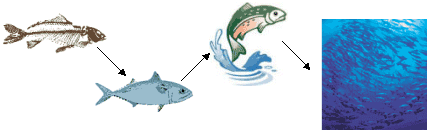
\includegraphics[width=.6\textwidth]{mts-2.png}
\end{center}

Lebende Organismen, Individuen, können sich in einem Obersystem vereinen.
„Obersystem“ ist eine mehr oder weniger organisierte Gruppe von Tieren oder
Pflanzen, zum Beispiel, ein Bienenstock. Aber ein scharfer
qualitativen Sprung geschieht hier schon nicht mehr. 

In Analogie zu biologischen Systemen kann man den Begriff „Technisches System“
als eine besondere Hierarchieebene interpretieren, auf der das System die
Möglichkeit erhält, unabhängig zu handeln, d.h. die Ebene eines lebenden
Organismus.

Mit anderen Worten, das „Technische System“ entspricht in der Technik dem
Niveau des Organismus in der Natur. In einer Patentanmeldung wird das als
“Maschine arbeitet“ bezeichnet. Das heißt, „das System der technischen
Objekte“ plus ein menschlicher Operator. Zum Beispiel, ein ??\footnote{Hier
  steht \foreignlanguage{russian}{карбюратор} -- Vergaser, aber das ergibt
  keinen Sinn. HGG} ist kein TS, sondern einfach ein System, ein Satz
technischer Objekte. Und der Mann, der mit dem ?? auf die Nuss klopft, das ist
ein TS mit einer nützlichen Funktion: die Nüsse von den Schalen zu reinigen.
Genauso ist ein Mann mit einer Hacke ein TS, ein Traktor mit einem Pflug aber
nicht. Paradox ...

\emph{“Mensch“ -- was ist das in Bezug auf das Technische System? Was daran
  ist schwierig zu verstehen? }

Wahrscheinlich wird die Verwirrung durch die Formulierung der Frage selbst
verursacht.  Psychologisch ist es schwer, einen Menschen und eine Bremsbacke
auf die gleiche Stufe zu stellen.

Es besteht kein Zweifel daran, dass der Mensch als Teil der Technosphäre die
direkteste Beziehung zu jedem beliebigen TS hat und kann zu diesem in den
folgenden Rollen stehen:
\emph{Im Obersystem:} 
\begin{itemize}\itemsep0pt
\item[1.] als Benutzer. 
\item[2.] als Entwickler. 
\item[3.] als Hersteller der technischen Objekte des Systems. 
\item[4.] als Person, welche die technische Wartung, Reparatur und das
  Recycling der technischen Objekte des Systems absichert.
\end{itemize}
\emph{Im System:} 
\begin{itemize}\itemsep0pt
\item[1.] als Operator, dem Hauptelement des Steuerungssystems. 
\item[2.] als Energiequelle. 
\item[3.] als Antrieb. 
\item[4.] als Transmission. 
\item[5.] als Arbeitsorgan. 
\item[6.] als bearbeitetes Objekt. 
\end{itemize}
\emph{In der Umwelt:} 
\begin{itemize}\itemsep0pt
\item[1.] als Element der Umwelt. 
\end{itemize}
Der Anwender ist zweifelsohne die Hauptperson. Er ist derjenige, der für die
Erstellung des TS bezahlt, nach seinem Willen setzen sich die Entwickler und
Hersteller an die Arbeit. Er bezahlt die Arbeit des Operators, die technische
Wartung, Reparatur und das Recycling der technischen Objekte des Systems.

Die zweite Personengruppe sorgt für das Funktionieren des TS bei der Arbeit,
erfährt dessen Aktionen an sich selbst.

Die dritte Gruppe unterstützt oder behindert diesen Prozess indirekt, oder
beobachtet ihn einfach und ist den Nebenwirkungen ausgesetzt, die bei der
Arbeit des TS entstehen.

Eine Person kann mehrere Rollen gleichzeitig ausüben. Zum Beispiel als Fahrer
des eigenes Autos oder als Person, die einen Inhalator benutzt. Oder als
Radfahrer.  Jener ist Element fast aller Systeme des Fahrrads mit Ausnahme des
Arbeitsorgans (Sitz) und der Transmission (Räder und Fahrradrahmen).

\emph{Trotzdem, es stellt sich heraus, dass der Mensch ein obligatorischer
  Teil eines Technischen Systems ist.}

Man sollte meinen, was macht das für einen Unterschied. Denn wenn es um die
Sache geht, um das Lösen realer Ingenieur-Aufgaben, dann wird der Mensch
schnell aus dem Problem ausgeklammert und es wird auf der Ebene des
Untersystems gearbeitet. Ja, aber nur dort, wo Harmonisierung und
Energiedurchsatz zwischen Subsystemen erfolgt, die in keiner Weise mit dem
Operator verbunden sind. Sobald wir uns dem Kontrollsystem nähern, steht das
Problem der Interaktion zwischen Mensch und technischen Objekten in voller
Größe.

Nehmen Sie zum Beispiel das Auto. Das Auto hat sein heutiges Aussehen bereits
in den späten 1970er Jahren erhalten, als die Airbags erfunden wurden und
zuverlässige Automatikgetriebe. Die meisten Neuerungen seit dieser Zeit.
zielen nur darauf ab, Steuerung, Sicherheit und Komfort von Wartung und
Reparatur zu verbessern, d.h. auf die Interaktion des Menschen als Hauptteil
des TS mit den anderen Teilen.

Der Lastwagen der 40-50er Jahre hatte ein Lenkrad mit einem Durchmesser von 80
cm.  Der Fahrer muss sehr stark zu sein, um ein solches Fahrzeug zu fahren.
Und in der Luftfahrt ...  das Riesenflugzeug aus den 30er Jahren „Maxim
Gorki“.  Um ein Manöver auszuführen, mussten der erste und zweite Piloten
zusammenziehen am Steuerknüppel ziehen. Manchmal riefen sie noch den Navigator
und den Rest der Besatzung zur Hilfe. Heute kann ein Operator mit Verstärkern
viel stärker beladene Mechanismen steuern. Es scheint, das Problem ist gelöst.
Ah nein, man vergisst oft wieder den Menschen ... Die Sache ist so, dass die
Verstärker es dem Operator nicht immer erlauben, das Verhalten des gesteuerten
Mechanismus vollständig zu spüren.  Manchmal führt das zu Havarien.

Zum Beispiel das Problem der Verkehrssicherheit eines Autos oder das noch
„eintönigere“ Problem der Steuerung einer Lokomotive. Hier ist es sehr
wichtig, dass der Operator immer in einem wachen, handlungsfähigen Zustand
ist.  Auch dieses Problem wird im Obersystem gelöst -- die Ursachen für das
Einschlafen am Steuer werden beseitigt, eine medizinische Überwachung wird
durchgeführt, die Verantwortung des Fahrers als Operator steigt. Aber immer
öfter wird das direkt im Technischen System geregelt. Direkt im Cockpit. Wenn
der Maschinist nicht rechtzeitig eine Signallampe ausschaltet, wird der Motor
abgeschaltet und der Zug hält an.  Oder im Auto: es fährt erst, wenn man sich
angeschnallt hat.  D.h. es gibt Rückkopplungen wie zwischen allen anderen
Elementen des TS auch.

Vielleicht ist einer der Gründe dafür, warum diese Richtung der Verbesserung
technischer Systeme erst in den letzten Jahren begonnen hat, sich aktiv zu
entwickeln, das Unverständnis über den Platz des Menschen in dieser Struktur.
Oder, besser gesagt, nicht so sehr Unverständnis ...  Allgemein gerät der
Entwickler in eine komplizierte psychologische Situation. Ein Mensch, der neue
Dinge entwickelt, fühlt sich zu Recht als Schöpfer. Er kann nicht bis zu Ende
fühlen, dass ein genau solcher Mensch auch Operator, Antrieb oder Arbeitsorgan
als Teil des Mechanismus, der Maschine, des Technischen Systems sein kann.
Das wird noch nicht deutlich, wenn es sich um ein weit verbreitetes TS
handelt, das eng mit Menschen interagiert, wie ein Auto. Hier kann der Mensch
gleichzeitig Entwickler, Betreiber und Benutzer sein.

Genau wie mit dem Computer. Es ist schwierig, mit den meisten
Computerprogrammen zu arbeiten, selbst jetzt, wo die Entwickler die einfache
Wahrheit verstanden haben, dass mit dem Programm ein menschlicher Operator
arbeitet, dem das Ergebnis und nicht der innere Aufbau des Programms
interessiert.  Jetzt gibt es solche Begriffe wie „benutzerfreundliche
Schnittstelle“.  Aber früher ... Warum weit gehen, denken Sie an ein
„Lexikon“.

Und andere TS, die auf den ersten Blick weit entfernt von Menschen operieren
.... Sie gibt es haufenweise.  Oft kommt einem dabei gar nicht in den Sinn,
dass der Mensch auch Teil solcher Technischer Systeme ist.  Aber es ist doch
so, dass bei der Entwicklung jedes von ihnen das Zusammenwirken der Elemente,
aus denen es aufgebaut ist, unter Berücksichtigung der Möglichkeiten des
menschlichen Körpers und Verstands zu analysieren war. Manchmal ist das nicht
erfüllt.

Mehr noch, oft werden viele der heute bekannten natürlichen Faktoren
ignoriert, die das Wohlbefinden des Menschen die Klarheit seiner Bewegungen
und seine Reaktionsgeschwindigkeit beeinflussen. Und wie ist es mit neu
entdeckten psychologischen Faktoren, wie dem „Kassandra-Effekt“ [10]?

Und es erhebt sich als furchterregender Pilz Tschernobyl, Flugzeuge stürzen ab
und Schiffe kollidieren.

\emph{Und was brauchen Sie außer einem Operator noch für ein betriebsbereites
  technisches System?}

\section*{Der vollständige Bestand eines minimal funktionsfähiges technisches
  System.} 

Es gibt eine Reihe von technischen Objekten, die in das System integriert
sind, sowie den menschlichen Operator. Reicht das aus, damit das Technische
System seine nützliche Funktion erfüllt und das Bedürfnis des Benutzers
befriedigt, oder braucht es mehr?

Erinnern wir uns an das berühmte TRIZ-Beispiel, das im Buch von G. Ivanov [11]
angeführt wird. Es geht um den russischen Wissenschaftler Kapitza, der ein
Werk von Simmens und Schuckert besucht, das Generatoren produziert. Die Herren
des Werks zeigten ihm einen Generator, der nicht arbeiten wollte und boten
1\,000 Mark für dessen Reparatur an. Kapitza hat schnell bemerkt, dass die
zentrale Lagerung schief und verklemmt war, griff zum Hammer und schlug auf
den Lagerkörper ein -- der Generator läuft.

Die verwirrten Auftraggeber baten um eine Rechnung für die geleistete Arbeit.
Kapitza schrieb: \emph{1 Schlag mit dem Hammer -- 1 Mark, für das Wissen,
  wohin man schlagen muss -- 999 Mark.}

Und hier ist ein weiteres Beispiel von Fenimore Cooper [12].

Die Helden der Geschichte rannten vor den Verfolgern davon, die Indianer
stellten sie im Dickicht hohen trockenen Grases und zündeten dieses an.  Die
Feuerwand bewegt sich, was tun? Der alte Jäger geriet nicht in Panik und
steckte das Gras in der Nähe ihres Standorts in Brand. Die Feuerwand bewegte
sich auf die andere Feuerwand zu und verbrannte den Brennstoff für das andere
Feuer.  Das Feuer ging aus, die Flüchtigen konnten sich retten.

Was ist das Technische System in dem einen und in dem anderen Fall?

Im ersten Beispiel. Der Nutzer möchte den Generator starten.  Die nützliche
Funktion ist die Ausrichtung des Lagers. Der Operator ist Kapitza, das System
technischer Objekte - ein Hammer.

Es ergibt sich, dass das Technische System Kaitza mit einem Hammer ist.

Im zweiten Beispiel. Das Bedürfnis des Nutzer ist es, das Feuer zu stoppen.
Die nützliche Funktion besteht darin, das Gras zu vernichten (als Brennstoff
für das entgegenkommende Feuer). Operator - der alte Jäger, das System 
technischer Objekte - Feuerstein und die Flamme.

Das Technische System ist der Jäger mit Feuerstein und Flamme.

Was geht hier also vor sich? Eine vernachlässigbar kleine Handlung eines
Menschen als Operator mit Hilfe primitiver technischer Mittel resultierten in
einem so großartigen Ergebnis im ersten wie im zweiten Fall! Ist das wirklich
alles?  Ist das wirklich der vollständige Bestand der technischen Systeme, die
es im ersten Fall ermöglichten, eine riesigen Generator in Betrieb zu setzen,
und im zweiten, die Feuerwand zu stoppen?

Nein, das ist nicht so.

Das Wichtigste -- das, was in der vorangegangenen Argumentation völlig
übersehen wurde -- ist die Informationskomponente.

In der Tat, man kann morgens bis abends ergebnislos mit einem Hammer auf dem
Generator herumschlagen. Und Kapitza hat nicht irgendwie geschlagen, sondern
auf eine streng definierte Weise. Und darin.  In seinem Fall bestand die
Informationsunterstützung für seine Aktionen aus zwei Teilen: „die Fähigkeit,
mit dem Hammer zu klopfen“ und das Wissen, das Verständnis, „wo genau“ man
zuschlagen muss.

Genauso hätte man das Gras ohne jeden Verstand auf viele Weisen in Brand
setzen können, und die meisten dieser Optionen würden für den Brandstifter
selbst schlecht ausgehen.

Wenn wir das zweite Beispiel weiter analysieren, so wird deutlich, dass
trockenes Gras in Brand zu setzen Sinn macht, wenn der Jäger nicht nur weiß,
dass der Wind das Feuer dem anderen Feuer entgegen jagt, sondern dieser Wind
aus der richtigen Richtung auch verfügbar ist.

Daher ist sehr wichtig zu wissen, „wie man es macht“, wie die nützliche
Funktion ausführen, unter Verwendung technischer Objekte und verfügbarer
Stoff-Feld-Ressourcen, die für die Dauer der arbeit ebenfalls Teil des TS
werden.

Für die Vervollständigung zu einem vollen minimal arbeitsfähigen TS ist es
notwendig, die folgenden informationellen und materiellen Bestandteile zu
berücksichtigen:
\begin{itemize}\itemsep0pt
\item[1.] Den technologischen Prozess der Ausführung der nützlichen Funktion.
\item[2.] Die materiellen technischen und natürlichen Objekte und Systeme auf
  verschiedenen Hierarchieebenen.
\item[3.] Einen oder mehrere Operatoren, die eine Reihe von Fertigkeiten zur
  Steuerung materieller Objekte und Systeme haben.
\item[4.] Stoffe und Felder, die zum Betrieb der materiellen Objekte und
  Systeme erforderlich sind, sowie deren Arbeitsprodukte.
\item[5.]  Stoffe und Felder, die für das Funktionieren des Operators
  erforderlich sind, und deren Arbeitsprodukte.
\item[6.] Das bearbeitete Objekt (in einzelnen Fällen).
\end{itemize}
Vollständige Zusammensetzung eines Technischen Systems:\footnote{Die Abbildung
  muss noch ins Deutsche übertragen werden -- HGG.}
\begin{center}
 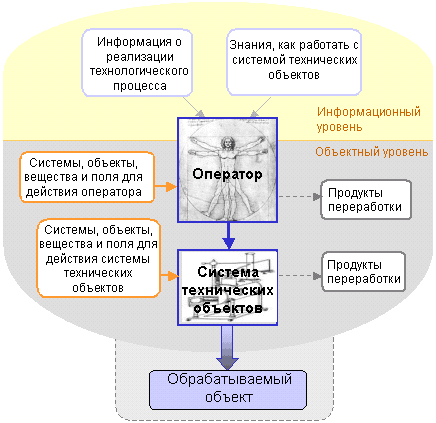
\includegraphics[width=.8\textwidth]{mts-3.png}
\end{center}
Erst in dieser Struktur erhält das TS die Möglichkeit, überall und an jedem
Ort völlig autonom zu arbeiten. Auch in der Schwerelosigkeit und im luftleeren
Raum.

Dieser Ansatz -- die Ausstattung des TS mit allem, was für seine nützliche
Funktion erforderlich ist -- entwertet den traditionellen, sehr bequemen
Ansatz nicht, alles zur Erfüllung einer Funktion Notwendige in ein System
einzusammeln und dieses zu transformieren, indem es gedanklich vom Obersystem
getrennt wird. Jede Arbeit ist einfacher auszuführen, wenn man vorher alle
notwendigen Materialien, Werkzeuge und Zeichnungen vorbereitet, diese auf
bequeme Art und Weise bereitlegt, um später nicht in der „Werkstatt“ (dem
Obersystem) herumzuwühlen, wenn man sich daran erinnert, was für die
Arbeitsfähigkeit unseres TS noch benötigt wird.

Das heißt, das Technische System ist das Obersystem des Systems technischer
(materieller) Objekte.

Dieses Verständnis eines TS korrespondiert mit der Beschreibung, die
N. Matvienko [8] gibt: 
\begin{quote}\bf
  “Jedes Technische System ist eine Gesamtheit materieller, energetischer und
  informationeller Elemente (mit anderen Worten -- materieller Teile und
  Details, energetischer Ressourcen für deren Funktionieren und einer Sammlung
  von Vorschriften, Anweisungen, Befehlen, Signalen, welche die Abfolge sowie
  Art und Weise der Interaktion materieller Elemente mit den umgebenden
  Systemen und zwischen sich selbst bestimmen)“.
\end{quote}
In diesem Ansatz ist der menschliche Operator der Mittelpunkt, die Basis des
Technischen Systems.

Dabei kann ein von Menschen organisiertes „Technisches System“ die Verwendung
von materiellen technischen oder natürlichen Objekten umfassen -- zum Beispiel
Akupunktur oder Gütertransport --, oder ganz ohne sie auskommen -- die Rede
eines Anwalts vor Gericht oder ein Tanz. Das macht manchmal keinen großen
Unterschied.  Als Beispiel für diese Behauptung kann der Anwalt dienen, der im
Gerichtssaal mit einem Mikrofon oder ohne dieses spricht.

Und, wenn man es genauer betrachtet, ist der Mensch selbst ein
multifunktionales Technisches System. Die Natur des Menschen ist eine
zweifache Einheit -- er hat die Fähigkeit zu denken, seine Handlungen zu
modellieren, Entscheidungen zu treffen. Und zu handeln, indem er seinen Körper
für irgendeine Art von Arbeit einsetzt. Genau hier kommen die informationellen
und materiellen Bestandteile des Menschen zu einer Einheit zusammen.

Der Mensch als Operator hat alle wesentlichen Teile eines TS und kann, die
informationelle und materielle Absicherung vorausgesetzt, irgendwelche
Funktionen erfüllen, indem der diese mit den Fähigkeiten seines Körpers
abgleicht. Wenn diese Möglichkeiten ausgeschöpft sind, ist es möglich, den
Körper mit materiellen Objekten zu ergänzen, sie in Systeme zu integrieren und
so die Möglichkeiten des Menschen zu erweitern. Es beginnt der normale Prozess
der Entfaltung eines Technischen Systems.  Stein, Stock, Schaufel, Bagger ...
Der Mensch wird immer stärker, kann ein immer größeres Arbeitsvolumen
bewältigen.

Was ist mit Trimmen\footnote{Im Russischen gibt es ein Gegensatzpaar
  „entfalten -- einfalten“, das im TRIZ eine sehr wichtige Rolle spielt,
  zuletzt aber immer stärker nur das „Einfalten“, ins Englische und Deutsche
  als „Trimmen“ übersetzt.  Eine sehr unglückliche Üersetzung -- HGG}?
Schließlich scheint man den Menschen nicht „trimmen“ zu können. Ja, wenn man
vom Trimmen von Objekten spricht. Aber hier geht es um Trimmen auf der
informationellen Ebene.

Es ist zum Beispiel an der Zeit, im Garten zu gießen. Wir könnten die
Gießkanne nehmen, einen Schlauch anschließen, oder eine ganze
Bewässerungsmaschine aufstellen. Oder Sie könnten einfach in den Himmel
schauen und, wenn es bald regnen wird, ist nichts zu tun. Das heißt, das
Trimmen geschieht auf der Ebene der Funktionen, der technologischen
Operationen. Letztlich auf der Ebene der Planung von Systemen und Prozessen.
Eine logische Anwendung dieser Richtung ist die TRIZ selbst. Schließlich sind
die Begriffe „ideal“, „ideales Endergebnis“ eines der Grundkonzepte dieser
Methodik.

Das wurde vor langer Zeit bemerkt, und selten kommt ein Märchen ohne etwas
aus, das sich „von selbst“ erledigt, der Mensch erreicht ein Ergebnis ohne
jede Aufwendung.  Mit der Kraft des Gedanken sozusagen werden Berge versetzt,
kann man durch die Zeit und den Raum reisen.  Die „technische Aufgabe“ für die
Entwicklung des Menschen in dieser Richtung schreibt Fantasten und
Geschichtenerzähler vor. Und es gibt Grund zur Annahme, dass diese Richtung
gemeistert wird. Levitation, Bewegen von Objekten durch Blick, Verbindung über
große Entfernungen ohne alle technischen Mittel und vieles mehr -- kann dem
Menschen zugänglich sein.

Ja, das ist interessant, aber was gibt all das oben Gesagte für die
Transformation, die Verbesserung Technischer Systeme in der realen Praxis?

\section*{Starker Anstieg der Zahl der Ressourcen, die für
  Systemtransformationen angewendet werden können.} 

\emph{Im traditionellen Ansatz können die folgenden Ressourcen verwendet
  werden:}
\begin{itemize}\itemsep0pt
\item[1.] Das System selbst.
\item[2.] Seine Untersysteme.
\item[3.] Die Beziehungen zwischen Untersystemen.
\item[4.] Die Beziehungen zwischen den einzelnen Untersystemen und dem System.
\end{itemize}
\emph{Im hier vorgeschlagenen Ansatz, nimmt die Zahl der Ressourcen, die
  potenziell genutzt werden, dramatisch zu. Dies sind nur einige von ihnen: }
\begin{itemize}\itemsep0pt
\item[1.] Das technische System selbst.
\item[2.] Das technologische Verfahren.
\item[3.] Technologische Operationen.
\item[4.] Das System technischer Objekte.
\item[5.] Subsysteme des Systems der technischen Objekte.
\item[6.] Der Operator als denkendes System.
\item[7.] Der Körper des Operators als materielles biologisches System.
\item[8.] Die Sinnesorgane des Operators.
\item[9.] Das System der Fertigkeiten des Operators.
\item[10.] Einzelne Fertigkeiten des Operators.
\item[11.] Systeme, Objekte, Stoffe und Felder, die vom System der technische
  Objekte genutzt werden.
\item[12.] Systeme, Objekte, Stoffe und Felder, die vom Operator genutzt
  werden.
\item[13.] Beziehungen zwischen dem Technischen System und dem technologischen
  Prozess.
\item[14.] Beziehungen zwischen den technologischen Operationen und dem
  technologischen Prozess.
\item[15.] Beziehungen zwischen den technologischen Operationen.
\item[16.] Beziehungen zwischen dem Technischen System und den technologischen
  Operationen.
\item[17.] Wechselwirkung zwischen Stoffen und Feldern, die vom Technischen
  System über das System der technischen Objekte genutzt werden.
\item[18.] Wechselwirkung zwischen Stoffen und Feldern, die vom Technischen
  System über den Operator genutzt werden.
\item[19.] Beziehungen zwischen den Teilsystemen des Systems der technischen
  Objekte.
\item[20.] Beziehungen zwischen jedem der Subsysteme des Systems Materieller
  Objekte und dem System der technischen Objekte.
\item[21.] Beziehungen zwischen den Subsystemen des Systems der technischen
  Objekte und dem technologischen Prozess. \ldots
\end{itemize}
Es ist an der Zeit, einige Beispiele zu bringen. 

%% \begin{wrapfigure}{l}{.3\textwidth}
%% 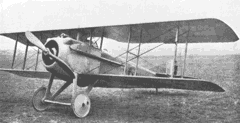
\includegraphics[width=.3\textwidth]{mts-4.png}
%% \end{wrapfigure}
\paragraph{1. Das klassische Flugzeug.}
Das klassische Flugzeug des frühen zwanzigsten Jahrhunderts -- das sind zwei
Flügel, die mit zahlreichen Streben und Seilen am Rumpf befestigt wurden.
Damit ein solche Flugzeug gut fliegen konnte (das war besonders wichtig für
Kampfflugzeuge), müssen die Spannseile richtig gespannt werden. Da sich die
Seile unter Last dehnen, mussten Spannungen oft mit Hilfe einfachster
Schraubmechanismen reguliert werden. An der Spannstrecke wurde ein Lineal
angebracht, und die Strecke mit einem Dynamometer herausgezogen. Über den Grad
der Spannung wurden anhand der Abweichung von der Geraden beurteilt. Dieser
Prozess war sehr mühsam und langsam.

Was tun? Wie den Prozess der Spannungs-Anpassung beschleunigen?

Im Kern war es notwendig, ein neues System zur Spannungsregulierung
auszudenken. Wenn die Löser dieser Aufgabe allein vom System der Materiellen
Objekte ausgegangen wären, die zur Erfüllung dieser Funktion verwendet wurden,
so wäre das extrem schwierig geworden.  Wenn man aber berücksichtigt, dass im
System auch ein Operator präsent ist, so erhöht sich die Zahl der möglichen
Transformationen signifikant. Und so kann man das Problem mit den
Sinnesorganen des Operators lösen.

%% \begin{wrapfigure}{l}{.1\textwidth}
%% 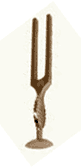
\includegraphics[width=.1\textwidth]{mts-5.png}
%% \end{wrapfigure}
In der Tat, warum nicht das Gehör nutzen, oder besser gesagt, Menschen mit
einem hohen tonalen Gehör? Klavierstimmer wurden eingeladen, die Dehnung
anzupassen, der Anpassungsprozess wurde um ein Vielfaches beschleunigt.

Interessant noch, da Klavierstimmer nicht genug waren, musste die folgende
Lösung gefunden werden, in der sich der in der TRIZ wiederholt beschriebene
Trend der „Verdrängung des Menschen aus TS“ abzeichnet. Die Dehnungskontrolle
wurde wieder an die Mechaniker abgegeben, sondern anstelle des schwerfälligen
Lineals und Dynamometers wurde eine auf einen entsprechenden Kammerton
geeichte Stimmgabel verwendet.

\paragraph{2. Die Öllampe.}
Es ist schwer vorzustellen, welch titanische Arbeit die Erfinder geleistet
haben, um Öllampe ordentlich zum Leuchten zu bringen. Das ganze Problem war
die schlechte Ölversorgung der Dochtspitze. Um den Fluss zu verbessern, wurden
zahlreiche Federvorrichtungen erfunden, die Druck im Ölbehälter erzeugen.
Verwendet wurden auch Pumpen, um die Ölversorgung zu erzwingen. D.h., die
Arbeit erfolgte im Rahmen des „Systems technischer Objekte“ -- man versuchte,
die Maschine zu verbessern.  Als die vollständige Zusammensetzung des TS
betrachtet wurde, wurde klar, dass das Problem nicht in der Konstruktion der
Lampe bestand, sondern im Brennmaterial.  Als das schlecht durch den Docht
absorbierbare Öl durch flüssiges Petroleum ersetzt wurde, waren alle Probleme
verschwunden.

\paragraph{3. Computer.}
Angenommen, Sie möchten Ihren Computer im Dunkeln benutzen. Wenn wir das
System der materiellen Objekte transformieren, dann kommt sofort die Idee
einer leuchtenden Tastatur, Lämpchen und so weiter. Wenn man über das
Technische System nachdenkt, dann liegt die Antwort auf der Hand -- der
Operator muss in der Lage sein, im Dunkeln zu tippen, muss die Tastenanordnung
auswendig kennen.

Was kann man zum Schluss sagen? Heute werden in der TRIZ und anderen
Innovationsmethodiken die Begriffe „Technisches System“, d.h. das System, das
irgendeine Funktion \textbf{ausübt}, und „System Technischer (materieller)
Objekte“, d.h. das System, das für eine gewisse Art von Funktionen
\textbf{vorgesehen} ist, nicht klar unterschieden. Indem ich mich so wenig wie
möglich in den Streit der „Spitzköpfe“ und „Flachköpfe“\footnote{Dies spielt
  auf ein Sujet in „Gullivers Reisen“ an, das ich interessanterweise
  \emph{nicht} nur in der russischen Wikipedia gefunden habe: Die Feindschaft
  zwischen Flachköpfen und Spitzköpfen ist eine allegorische Darstellung jeder
  sinnlosen Konfrontation aus ideologischen Gründen. Swift benutzte diese
  Allegorie für das Bild des Kampfes zwischen Katholiken und Protestanten, der
  die Geschichte Englands, Frankreichs und anderer Länder durch Kriege,
  Aufstände und Hinrichtungen prägte. -- HGG} einmischte, habe ich versucht,
mich in dieser Frage zu orientieren.

Ohne den Leser auffordern zu wollen, mir zuzustimmen, würde ich mich freuen,
wenn sich dieser Analyseversuch für ihn in irgendeiner Weise als nützlich
erweist.

Ich bin den Kollegen V. Lenyashin, G. Severinets, E. Novitskaya, N. Khomenko
für ihre Hilfe bei Vorbereitung dieses Materials und für die schonungslose
Kritik der erste Version des Artikels durch W. Sibirjakow sehr dankbar.

\section*{Literatur}
\begin{itemize}
\item[1.] B.R. Gaines. General System research: Quo vadis? General System.
  Yearboor, 24, 1979.
\item[2.] A.A. Bogdanov. \foreignlanguage{russian}{Всеобщая организационная
  наука. Тектология} (Allgemeine Organisationswissenschaft. Tektologie). Buch
  1.  Moskau 1989.
\item[3.] G.S. Altschuller. \foreignlanguage{russian}{Творчество как точная
  наука} (Kreativität als exakte Wissenschaft).
  \url{http://www.trizminsk.org/r/4117.htm#05}.
\item[4.] A.F. Kamenyev. \foreignlanguage{russian}{Технические
  Системы. Закономерности развития} (Technische Systeme. Gesetzmäßigkeiten der
  Entwicklung).  Leningrad, Mashinostroenie 1985.
\item[5.] G. Altschuller, B. Zlotin, A. Zusman. V. Filatov.
  \foreignlanguage{russian}{Поиск новых идей: от озарения к технологии} (Suche
  nach neuen Ideen: von der Erleuchtung zur Technologie). Chisinau, Carta
  Moldaveniasca, 1989. S. 365.
\item[6.] V. Korolev. Über den Begriff „System“. Enzyklopädie der TRIZ.
 \url{http://triz.port5.com/data/w24.html}.
\item[7.] V. Korolev. \foreignlanguage{russian}{О понятии «система»} (Über den
  Begriff „System“) (2).  TRIZ-Enzyklo"|pädie.
  \url{http://triz.port5.com/data/w108.html}.
\item[8.] N.N. Matvienko. \foreignlanguage{russian}{Термины ТРИЗ} (Begriffe
  der TRIZ, eine Problemsammlung). Wladiwostok, 1991.
\item[9.] Y.P. Salamatov. \foreignlanguage{russian}{Система законов развития
  техники (Основы теории развития Технических систем)} -- System der Gesetze
  der Technikentwicklung (Grundlagen einer Theorie der Entwicklung technischer
  Systeme). Institut für innovative Gestaltung. Krasnojarsk, 1996.
  \url{http://www.trizminsk.org/e/21101000.htm}.
\item[10.] V.A. Sviridov. \foreignlanguage{russian}{Человеческий фактор} (Der
  menschliche Faktor).  \url{http://www.rusavia.spb.ru/digest/sv/sv.html}.
\item[11.] G.I. Iwanow. \foreignlanguage{russian}{Формулы творчества или как
  научиться изобретать} (Formeln der Kreativität oder wie man lernt zu
  erfinden).  Moskau. Prosveshtchenie. 1994
\item[12.] F. Cooper. Prärie. 
\end{itemize}

\end{document}
